\frame{
\frametitle{Why Topological Data Analysis?}
\framesubtitle{``Data has shape and the shape matters.'' - Gunnar Carlsson}
\begin{block}{}
 Today, Data is high-dimensional, \onslide<2->{HUGE,}
 \onslide<3->{present everywhere}
 \vspace{.2in}
 \begin{columns}
  \column{.32\textwidth}
 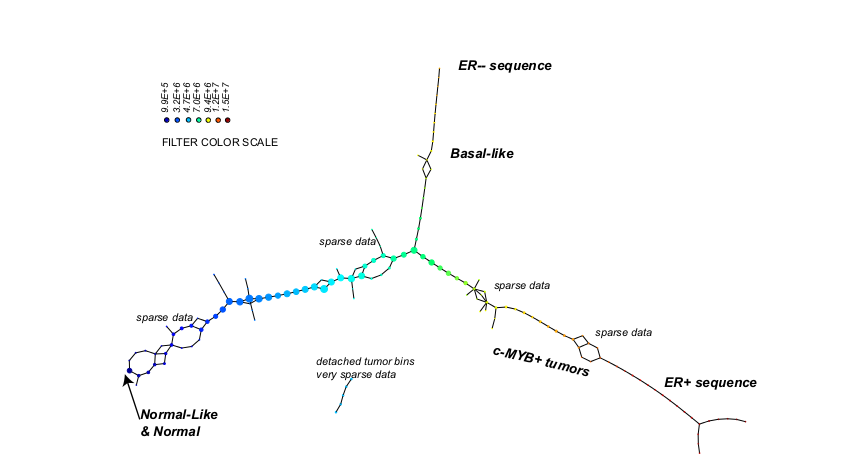
\includegraphics[width=\textwidth,height=1.25in]{examples/stanford-reeb}%
   \\
   ---------------------\\
   \scriptsize{Nicolaua, Levine, and Carlsson, PNAS 2011}
   \column{.32\textwidth}
   \onslide<2->{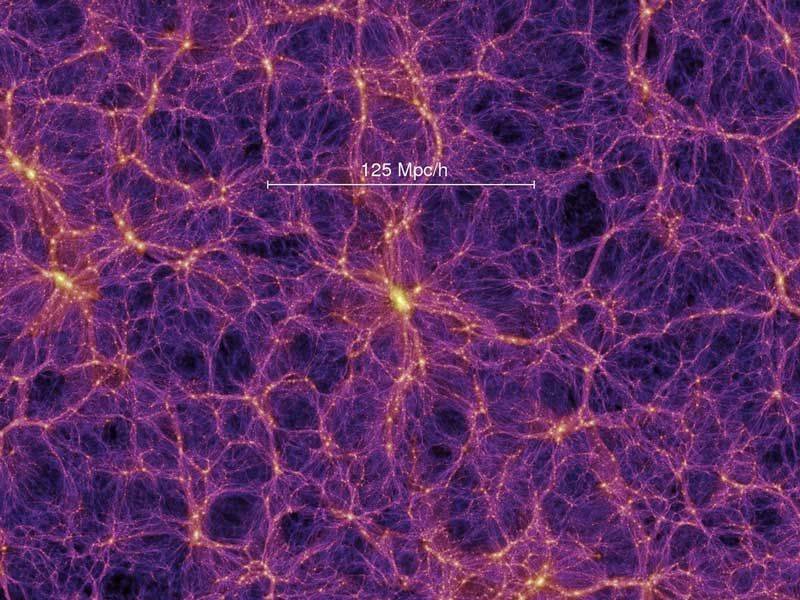
\includegraphics[width=\textwidth]{examples/cosmic-web}
   \\
   ---------------------\\
   \scriptsize{http://astrobites.com/}
   }%
   \column{.32\textwidth}
   \onslide<3->{
   \vspace{.2in} \\
   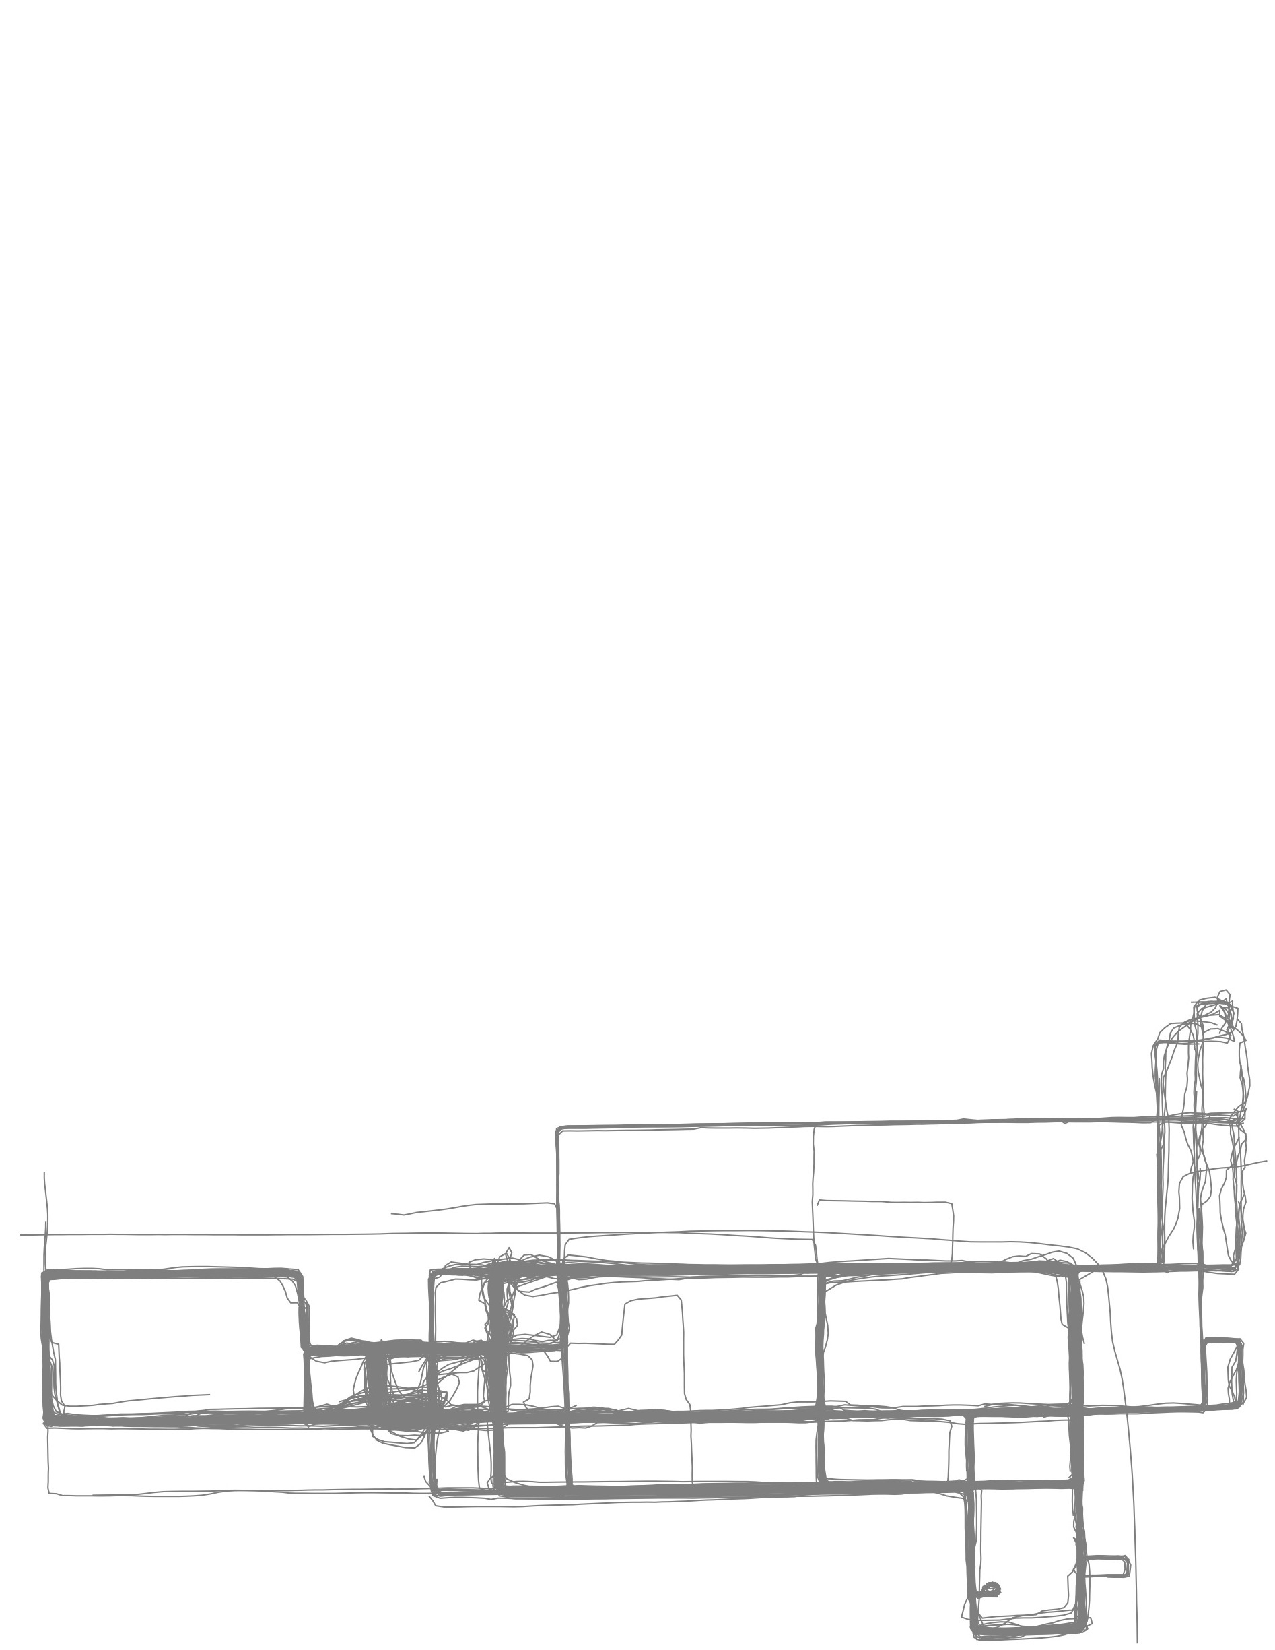
\includegraphics[width=\textwidth]{examples/chicago-tracks}
   \vspace{.2in} \\
   ---------------------\\
   \scriptsize{\url{www.mapconstruction.org}}
   }
 \end{columns}
 \vspace{.2in}
 ... and needs to be summarized, analyzed, and compared!

\end{block}
}

\frame{
    \begin{block}{\center{What questions do we ask in data anaylsis?}}
        \pause
    \begin{itemize}
        \item Think! Write down one question (2 min) \pause
        \item Pair! Share with partner, and add more questions to your list (5
            min) \pause
        \item Share! Raise hands please! (5 min) \pause
        \item More ideas? \url{mickas37@gmail.com}
    \end{itemize}
    \end{block}
}

\frame{
    \frametitle{Data Analysis Questions}
        \begin{block}{Summarize and Analyze}
            \begin{itemize}
                \item What is this shape? How many components / populations?
                    \pause
                \item Can we categorize? (Classification) \pause
                \item What are the parameters? (Inference: Point Estimation)
                    \pause
                \item How far do parameters likely lie from estimates?
                    (Confidence Sets) \pause
            \end{itemize}
        \end{block}
        \begin{block}{Compare}
            \begin{itemize}
                \item Are these the same (in distribution)? \pause
                \item Has something changed?  If so, what has changed? \pause
                \item Which is bigger? \pause
                \item Can we retain the null hypothesis? (Inference: Hypothesis
                    Testing) \pause
                \item What is the relationship between $X$ and $Y$? (Regression)
            \end{itemize}
        \end{block}
}

\frame{
    \frametitle{Most Important Questions}

    \pause
    \begin{block}{}
        1. Which descriptor best captures our data?
        \begin{itemize}
            \item Descriptors
            \item Confidence Sets
        \end{itemize}
    \end{block}

    \pause
    \begin{block}{}
        2. How do we measure distance between descriptors?
        \begin{itemize}
            \item Distances
            \item Clustering
        \end{itemize}
    \end{block}
}
